

\tikzstyle{cell} = [minimum height=0.6cm, minimum width=3cm,rectangle,style={fill=gray!20,draw,thick}]
\tikzstyle{muxn} = [minimum height=3.5cm, minimum width=0.6cm,rectangle,style={fill=gray!20,draw,thick}]
\tikzstyle{fil} = [->,style={thick}]
\tikzstyle{filb} = [style={thick}]

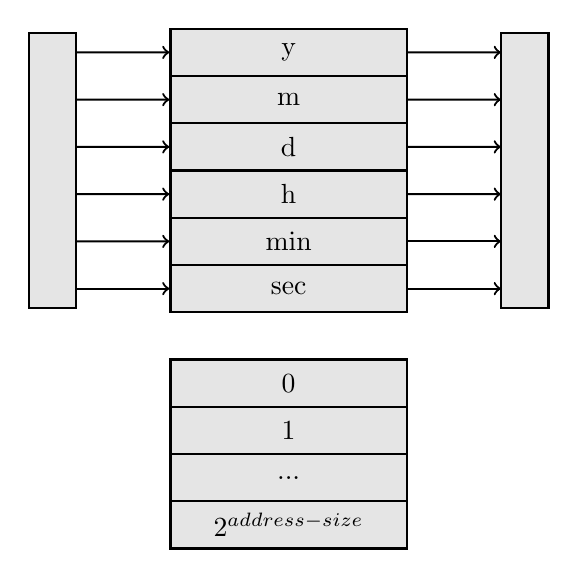
\begin{tikzpicture}[auto, scale = 0.6]
% Virtual cells	
	\node[cell] at (0cm,5cm) (y) {y};
	\node[cell] at (0cm,4cm) (m) {m};
	\node[cell] at (0cm,3cm) (d) {d};
	\node[cell] at (0cm,2cm) (h) {h};
	\node[cell] at (0cm,1cm) (min) {min};

% RAM cells
	\node[cell] at (0cm,0cm) (sec) {sec};
	\node[cell] at (0cm,-2cm) (Ram0) {0};
	\node[cell] at (0cm,-3cm) (Ram1) {1};
	\node[cell] at (0cm,-4cm) (dots) {...};
	\node[cell] at (0cm,-5cm) (Ram2n) {\(2^{address-	size}\)};

% Mux for virtual cells
	\node[muxn] at (-5cm,2.5cm) (muxn) {};
	\node at (-4.7cm,5cm) (muxny) {};
	\node at (-4.7cm,4cm) (muxnm) {};
	\node at (-4.7cm,3cm) (muxnd) {};
	\node at (-4.7cm,2cm) (muxnh) {};
	\node at (-4.7cm,1cm) (muxnmin) {};
	\node at (-4.7cm,0cm) (muxnsec) {};
	\draw[fil] (muxny) -- (y);
	\draw[fil] (muxnm) -- (m);
	\draw[fil] (muxnd) -- (d);
	\draw[fil] (muxnh) -- (h);
	\draw[fil] (muxnmin) -- (min);
	\draw[fil] (muxnsec) -- (sec);

% Demux for virtual cells
	\node[muxn] at (5cm,2.5cm) (demuxn) {};
	\node at (4.7cm,5cm) (demuxny) {};
	\node at (4.7cm,4cm) (demuxnm) {};
	\node at (4.7cm,3cm) (demuxnd) {};
	\node at (4.7cm,2cm) (demuxnh) {};
	\node at (4.7cm,1cm) (demuxnmin) {};
	\node at (4.7cm,0cm) (demuxnsec) {};
	\draw[fil] (y) -- (demuxny);
	\draw[fil] (m) -- (demuxnm);
	\draw[fil] (d) -- (demuxnd);
	\draw[fil] (h) -- (demuxnh);
	\draw[fil] (min) -- (demuxnmin);
	\draw[fil] (sec) -- (demuxnsec);

\end{tikzpicture}
